\documentclass[a4paper,english, 11pt]{article}

\usepackage[a4paper,inner=2.5cm,outer=2.5cm,top=2.5cm,bottom=2.5cm,pdftex]{geometry} 
\usepackage{graphicx}
\usepackage{titling}
\usepackage[colorlinks = true,
            linkcolor = blue,
            urlcolor  = blue,
            citecolor = blue,
            anchorcolor = blue]{hyperref}
\usepackage{enumerate}
\usepackage{fancyhdr}
\usepackage{lastpage}
\usepackage{tcolorbox}
\usepackage{booktabs} % For better table formatting
\usepackage{array} % for the 'p' column type
\hypersetup{colorlinks=true,linkcolor=blue, linktocpage}

\newcommand{\emailme}{\href{mailto:lukem@met.no}{lukem@met.no}}
\graphicspath{{Images/}} 

% header
\pagestyle{fancy}
\fancyhf{}
\fancyhfoffset[L]{1cm} % left extra length
\fancyhfoffset[R]{1cm} % right extra length
\rhead{\today}
\lhead{\bfseries How to create a Darwin Core Archive for scientists}
% footer
\rfoot{page \thepage\ of \pageref*{LastPage}}

% title
\title{How to create a Darwin Core Archive for scientists}
\date{\today}
\author{Luke Marsden (\emailme)}

\begin{document}

\maketitle
\tableofcontents
\newpage

\section{What is Darwin Core}
\label{s:dwc}

Darwin Core is a data standard originally developed for biodiversity informatics, though this has expanded to be useful for any type of data where you have data associated with one or a list of organisms. Darwin Core includes
\begin{itemize}
\item Darwin Core terms: A controlled vocabulary of terms - \url{https://dwc.tdwg.org/terms/}
\item Darwin Core Archive: A FAIR-compliant data format
\end{itemize} 

\section{What is a Darwin Core Archive}
\label{s:dwca}

A Darwin Core Archive (DwCA) is a self-describing dataset for taxonomic (species) data, sampling event data and associated traits or measurements. It consists of one or more data tables (CSV files) and 2 XML files, one (meta.xml) that describes how the files are organised and a second  (eml.xml) that provides the metadata describing the dataset as a whole. They are zipped together to create the Darwin Core Archive (DwCA) (Figure \ref{fig:dwca}). Don't worry if you don't know what an XML file is. You don't need to create this yourself. This is done for you using the Integrated Publishing toolkit as described in section \ref{ss:csv2dwca}.

\begin{figure}[htb]
    \tcbox[colback=white]{
    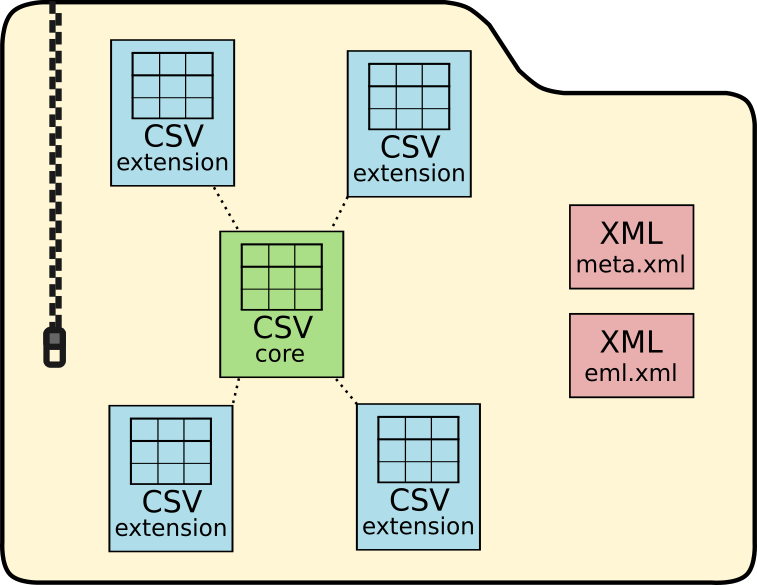
\includegraphics[width=0.7\textwidth]{dwca.png}
    }
    \caption{\label{fig:dwca}
        Visualisation of a Darwin Core Archive, portrayed using the star schema. The
        central event core can be surrounded by zero or many extension tables.
        It also contains a meta.xml file that describes what columns each CSV contains and links them to the term in a controlled volcabulary, and an eml.xml file that provides metadata that describes the dataset as a whole. They are zipped together to create a Darwin Core Archive.
    }
\end{figure}

Each CSV file contains a number of rows, and every row has its own unique ID (Figure \ref{fig:csvs}). These IDs are used to link the CSV files together. Every row in every \textit{extension} CSV file must include the ID of one row in the \textit{core} CSV file. This is called the \textit{star schema} and you can think of the core as the centre of the star. Note that a DwCA can only include a single level of extensions. In other words, one cannot include an extension to an extension file.

\begin{figure}[htb]
    \tcbox[colback=white]{
    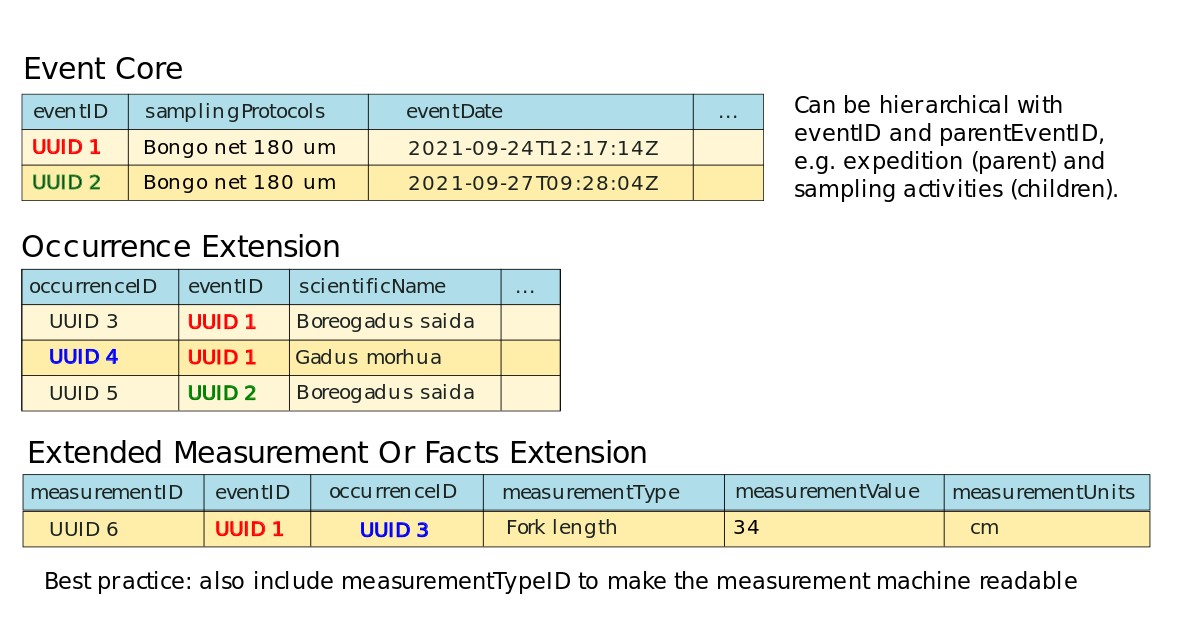
\includegraphics[width=1.0\textwidth]{example_dwca.png}
    }
    \caption{\label{fig:csvs}
        Example of a Darwin Core Archive with an Event Core and 2 extensions; an Occurrence Extension and a Extended Measurement Or Facts Extension. Note that this example does not include all the required columns for each core or extension. 
    }
\end{figure}

For more information on DwCA, see \url{https://ipt.gbif.org/manual/en/ipt/2.5/dwca-guide}.

Visual learners might want to watch this video about DwCAs: \url{https://www.youtube.com/watch?v=1Fuq8VZW_4c}


\subsection{Why do we use multiple CSV files?}
\label{ss:multiplefiles}

This is a common question, but we are not trying to make things needlessly complicated! This allows many-to-one relationships to be logged, for example multiple occurrences (observations of an organism or group of the same organism) logged for a single sampling event.

This method is also more efficient. The metadata related to the sampling event (coordinates, date, time etc) only needs to be logged once per sampling event instead of for each occurrence. This can save a lot of time and space, particularly if you have a lot of occurrences for each sampling event!

\section{Darwin Core terms and other controlled vocabularies}
\label{s:dwcterms}

Darwin Core includes a controlled vocabulary of terms for sharing information about biological diversity and associated data. Most (but not all) of the column headers you will include in your CSV files in your DwCA will be Darwin Core terms. Other terms will be from other controlled vocabularies.

A full list of Darwin Core terms can be found at \url{https://dwc.tdwg.org/terms/}.

\section{GBIF, OBIS and a network of data}
\label{s:gbif}

There are a number of data centres and services that manage Darwin Core data. GBIF (Global Biodiversity Information Facility) is the largest. Most (all?) of the other Darwin Core services make their data available via GBIF as well as their own platform. So if you publish your data with any of the below services, your data will also be available via GBIF.

The table below is just a few of the relevant platforms that contribute to this network of data.

\begin{table}[h!]
\centering
\caption{A network of Darwin Core data. This table is just a small selection of the services available.}
\begin{tabular}{cp{6cm}p{6.5cm}}
\toprule
Name & Website       & Comment  \\
\midrule
OBIS       & \url{https://obis.org/} & Aims to include all marine data. The OBIS community have been pushing the DwC standards forwards to build better functionality for scientific data.      \\
iNaturalist       & \url{https://www.inaturalist.org/} & For citizen science, nature enthusiasts and researchers. Offer some great apps like Seek that you can use on your mobile phone for taking pictures, identifying the organism and publishing the data \url{https://www.inaturalist.org/pages/seek_app}     \\
Living Norway     & \url{https://livingnorway.no/} & Norwegian ecological data project     \\
Artsdatabanken  & \url{https://www.artsdatabanken.no/} &  Service for collecting, organizing, and disseminating data related to Norwegian flora and fauna \\
\bottomrule
\end{tabular}
\end{table} 

\section{Cores and extensions}
\label{s:cores and extensions}

Which cores and extensions should you include in your DwCA? 

For most scientific data, you should be include and `Event Core', where 1 row is 1 sampling event. This can also be hierarchical, using eventID and parentEventID (Figure \ref{fig:eventcore}). You can include as many levels in the hierarchy as you wish. Every extension should then also include an eventID column where you input the ID of the sampling event that the data are related to. Refer to the child if using parent-child relationships in your event core.
\\
\\
\url{https://rs.gbif.org/core/dwc_event_2022-02-02.xml}

\begin{figure}[htb]
    \tcbox[colback=white]{
    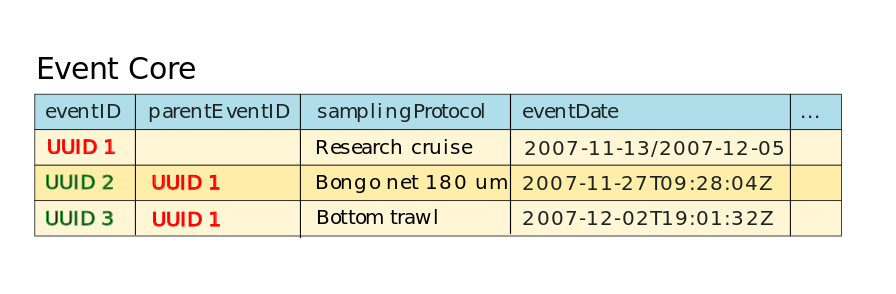
\includegraphics[width=1.0\textwidth]{example_event_core.png}
    }
    \caption{\label{fig:eventcore}
        Example of a hierarchical event core. The research cruise is the parent of the children sampling activities. This is shown using the eventID and parentEventID columns. 
    }
\end{figure}

You will most likely also have an occurrence extension, where one row is an observation of an organism of group of organisms of the same species.
\\
\\
\url{https://rs.gbif.org/core/dwc_occurrence_2022-02-02.xml}
\\
\\
Measurements related to the sampling event or occurrence (e.g. mass of your organism) go in an Extended Measurement or Facts extension.
\\
\\
\url{https://rs.gbif.org/extension/obis/extended_measurement_or_fact_2023-08-28.xml}
\\
\\
If you have material samples (soil, faeces) that you have taken your can log them using a Material Sample extension.
\\
\\
\url{https://rs.gbif.org/extension/ggbn/materialsample.xml}
\\
\\
If you have associated media you can refer to them using a Simple Multimedia Extension, and publish the media elsewhere. It is possible to publish these with GBIF too.
\\
\\
\url{http://rs.gbif.org/extension/gbif/1.0/multimedia.xml}
\\
\\
If you need to relate a row in one extension to a row in another extension, you can use the Resource Relationship Extension.
\\
\\
\url{https://rs.gbif.org/extension/dwc/resource_relationship_2022-02-02.xml}
\\
\\
And more extensions that are registered with GBIF can be found here.
\\
\\
\url{https://rs.gbif.org/extensions.html}

\section{Which columns are required in each extension?}
\label{s:required_columns}

It can be difficult to know which columns to include and what the minimum requirements are. Unfortunately, this information is not easy to find online. You can contact the data centre that you are publishing your data with.

Every core and extension should include an ID column that is specific to that extension or core (eventID for Event Core, occurrenceID for Occurrence Extension, measurementID for Extended Measurement or Facts Extension, etc). Every extension should also include the ID column for the core, e.g. if you have an Event Core, every extension must include an eventID column. Best practice is to use universally unique identifiers (UUIDs) for the IDs. You can generate them in most programming languages or using tools online such as \url{https://www.uuidgenerator.net/version4}.

I have also developed the Nansen Legacy spreadsheet template generator for Darwin Core Archives that has required and recommended columns for different cores and extensions included. Even if you would rather not use spreadsheets, you could use this to see which columns you should include.
\\
\\
\url{https://www.nordatanet.no/aen/template-generator/config%3DDarwin%20Core}
\\
\\
If you notice any issues with this or want to see something else added, please get in touch, or better still, raise an issue on GitHub.
\\
\\
\url{https://github.com/SIOS-Svalbard/Nansen_Legacy_template_generator}

\section{How to create a Darwin Core Archive}
\label{s:how}

To create a Darwin Core Archive you first have to create the CSV files. Then, you can use the Integrated Publishing Toolkit (IPT), developed by GBIF, to turn them into a Darwin Core Archive.

\subsection{Creating the CSV files}
\label{ss:CSVs}

You could use the Nansen Legacy template generator to help you with this. This will help you create a spreadsheet with a separate sheet for each core and extension (Figure \ref{fig:tg}). The descriptions for each term will appear as notes each time you select a cell to help you fill it in. I advise that you export each sheet to separate CSV files before you proceed with creating the Darwin Core Archive.

This video shows you how to use to template generator and how to publish the data afterwards: \url{https://www.youtube.com/watch?v=DbvlwnYXuPU}

\begin{figure}[htb]
    \tcbox[colback=white]{
    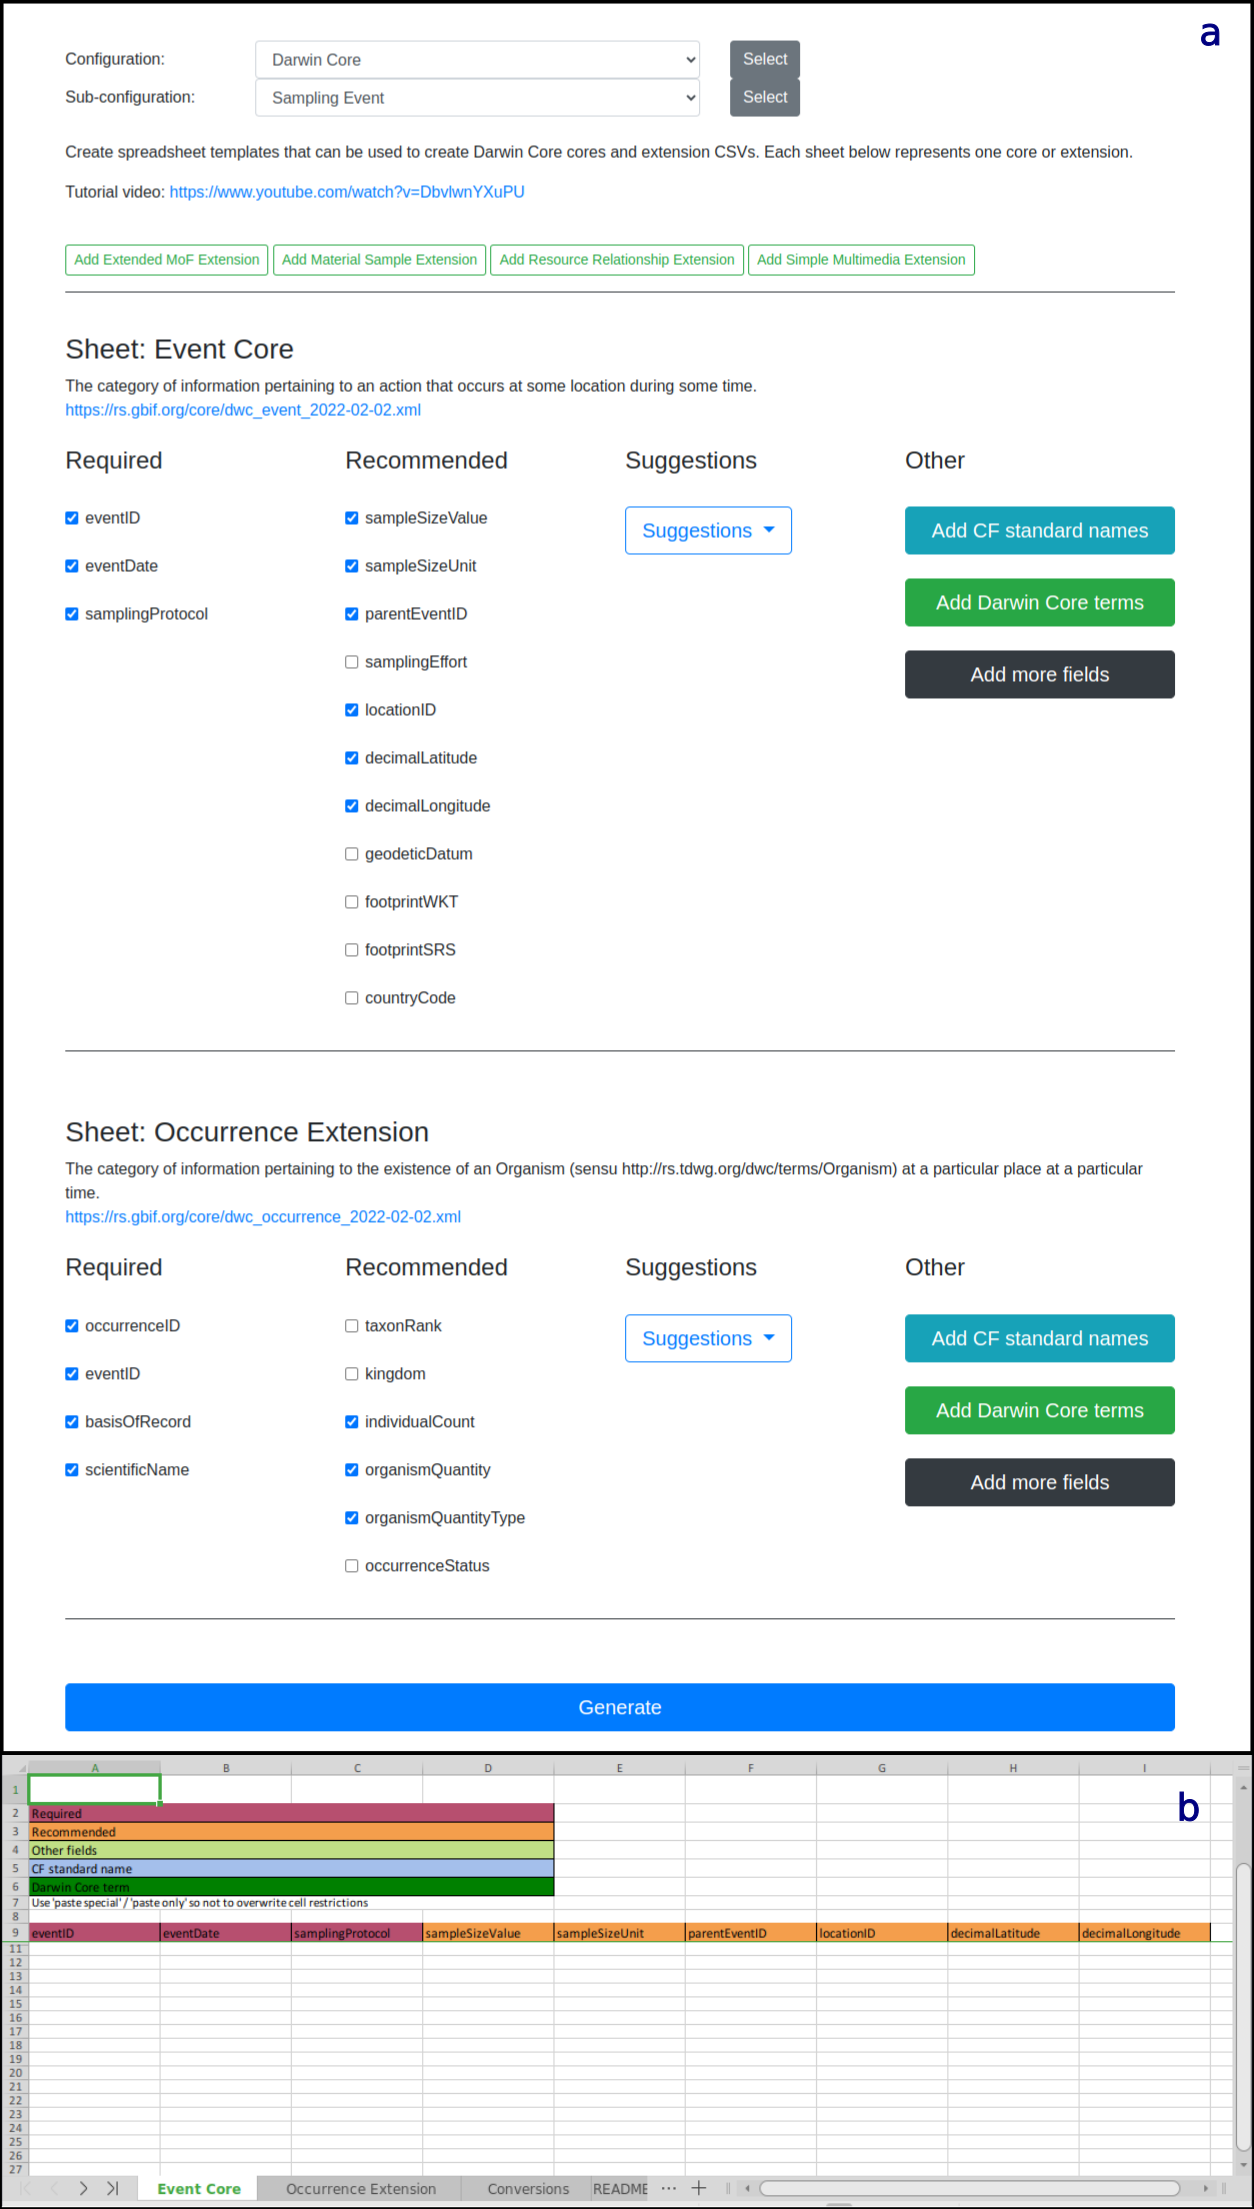
\includegraphics[width=0.8\textwidth]{tg.png}
    }
    \caption{\label{fig:tg}
        The Nansen Legacy template generator (a) and an example template (b)
    }
\end{figure}

Alternatively, you can create CSV files in any of way that you prefer. You can go to \url{https://rs.gbif.org/extensions.html} to see which cores and extensions you can use and which terms you can include in each. Note that it does not tell you which terms are required. This varies between data centres - GBIF has slightly different minimum requirements to OBIS for example for certain extensions.

\subsection{Creating a DwCA from your CSVs}
\label{ss:csv2dwca}

Once you have your CSV files, creating a DwCA is easy. You can using the Integrated Publishing Toolkit (IPT), developed by GBIF, to create the DwCA and also publish it.

Here is a map of places that have an IPT installed \url{https://www.gbif.org/ipt}. Choose one, contact them and ask for login details to their node.

For most people in Norway, good choices are the Norwegian Marine Data Centre (operated by IMR) - \href{mailto:datahjelp@imr.no }{datahjelp@imr.no}, or GBIF Norway - \href{mailto:helpdesk@gbif.no}{helpdesk@gbif.no}.

For how to use the IPT, watch the last 3 minutes of this video: \url{https://www.youtube.com/watch?v=DbvlwnYXuPU&t=280s}. The XML files are created through the IPT for you - you just need to upload your CSV files, select (map them to) which core or extension they are, and include metadata using a form.

This is a more extensive video tutorial on how to use the IPT created by GBIF (24 minutes): \url{https://www.youtube.com/watch?v=eDH9IoTrMVE}
 
\section{Making your data available via SIOS}
\label{s:sios}

Data relevant to Svalbard should be available via the SIOS data access portal \url{https://sios-svalbard.org/metsis/search?f%5B0%5D=dataset_level%3ALevel-1}

If you have published your data with the Norwegian Marine Data Centre, they contribute to SIOS so the data will be made available via the SIOS.

If you publish your data elsewhere (e.g. with GBIF Norway) you need to link your data to SIOS manually. You can use the metadata collection form on SIOS to do this. You will need to log in first. \url{https://sios-svalbard.org/metadata-collection-form}

\section{Citing your data in your paper}
\label{s:citing}

Cite your data just as you would cite any other scientific publication - in your list of references. You can also mention the data in a data availablity statement if your chosen journal requires one, but this should be as well as (not instead of) including the data in your list of references.

The recommended citation can be seen on the landing page of the dataset in the data centre you chose to publish with (GBIF or NMDC most likely).

\end{document} 